\documentclass[12pt]{article}

\usepackage{setspace}
\usepackage{caption}
\usepackage{subcaption}
\usepackage{float}
\usepackage{makecell}
\usepackage{amsmath}
\usepackage{graphicx}
\usepackage{subfig}
\graphicspath{ {./images/} }
\usepackage[utf8]{inputenc}
\usepackage[russian]{babel}
\usepackage{geometry}
 \geometry{
 a4paper,
 left=20mm,
 right=20mm,
 top=20mm,
 bot=20mm,
 }

\begin{document}

\begin{titlepage}
\begin{center}
    НАЦИОНАЛЬНЫЙ ИССЛЕДОВАТЕЛЬСКИЙ УНИВЕРСИТЕТ ИТМО \\
    Факультет систем управления и робототехники \\
    \vspace*{10\baselineskip}
    {\LARGEЭлектротехника} \\
    \ \\
    \ \\
    \begin{spacing}{1.5}
    {\large Лабораторная работа №5 \\
    ИССЛЕДОВАНИЕ ЭЛЕКТРИЧЕСКИХ ФИЛЬТРОВ \\
    \ \\
    Вариант 3R382}
    \end{spacing} \\
    \ \\
    \vspace*{10\baselineskip}
    \hfill {Студент: Кирбаба Д.Д.\ \ \ \ \ \ \ \ \ } \\
    \hfill {Группа: R3338\ \ \ \ \ \ \ \ \ \ \ \ \ \ \ \ \ \ \ \ \ } \\
    \hfill {Преподаватель: Китаев Ю.В.} \\
    \mbox{}
    \vfill {г. Санкт-Петербург\\2023}
\end{center}
\end{titlepage}

\subsection*{Цель работы}
Исследование исследование амплитудно-частотных характеристик (АЧХ) элетрических фильтров.

\subsection*{Ход работы}

\subsubsection*{RC фильтр нижних частот}
\begin{figure}[H]
    \centering
    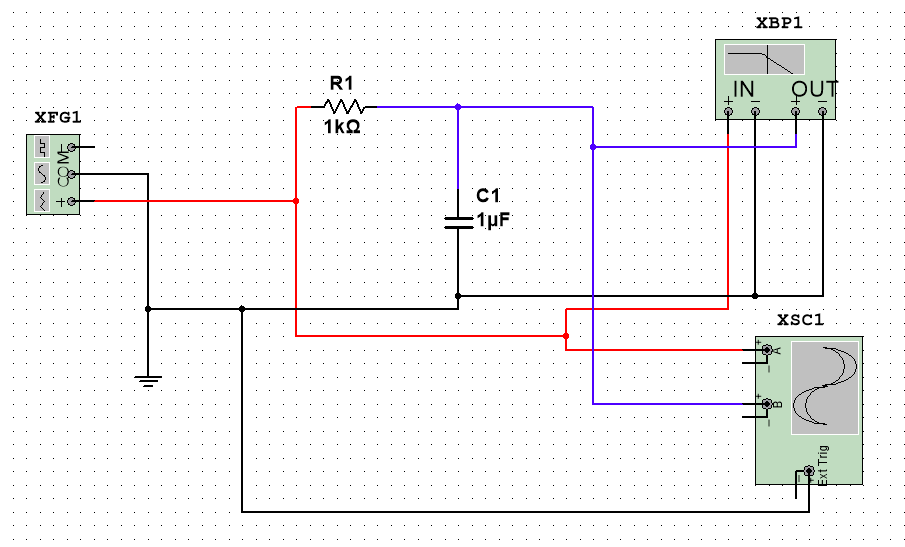
\includegraphics[width=0.5\textwidth]{1_scheme.png}
    \caption{Схема для исследования фильтра нижних частот RC.}
    \label{fig:1_scheme}
\end{figure}

На вход будем подавать синусоидальный сигнал с амплитудой $10 \ V$. \\

\begin{figure}[H]
    \centering
    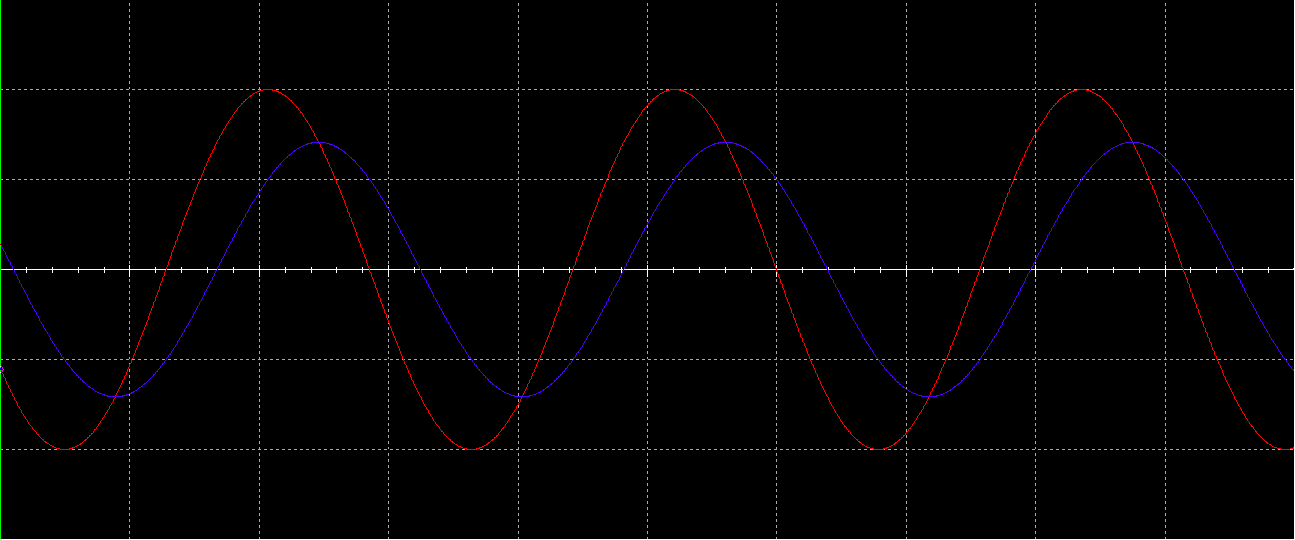
\includegraphics[width=\textwidth]{1_osc.png}
    \caption{Осциллограмма фильтра нижних частот.}
    \label{fig:1_osc}
\end{figure}

Теперь построим АЧХ и ФЧХ для данного фильтра. \\
Для этого изменяя частоту генератора синусоиды в диапазоне от $1 \ Hz$ до $100 \ kHz$ найдем 10 значений $V_{in}, \ V_{out}$ и вычислим коэффициент передачи фильтра для каждой пары и отметим данные экспериментально найденных точки на графике. \\
Также отметим частоту среза на графике и аналитически отобразим линии АЧХ и ФЧХ поверх экспериментальных точек.

\begin{figure}[H]
    \centering
    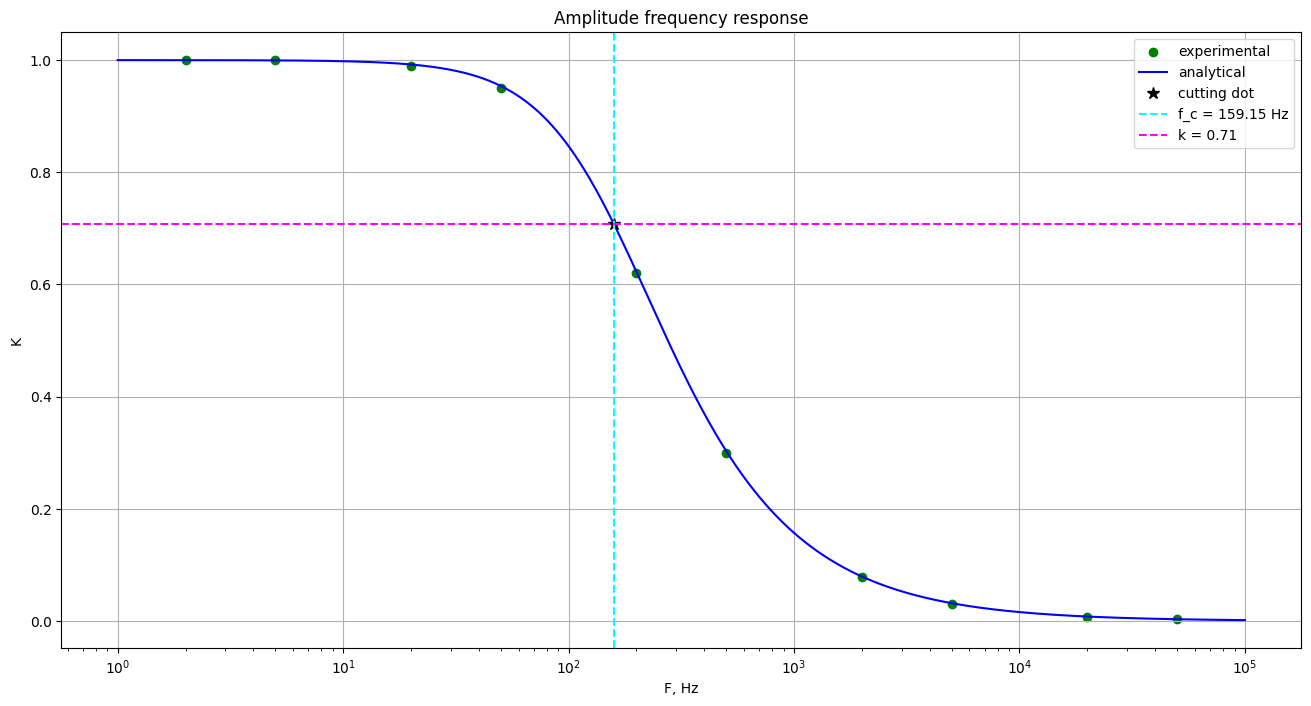
\includegraphics[width=\textwidth]{1_afr.png}
    \caption{Амплитудно частотная характеристика фильтра нижних частот.}
    \label{fig:1_afr}
\end{figure}

\begin{figure}[H]
    \centering
    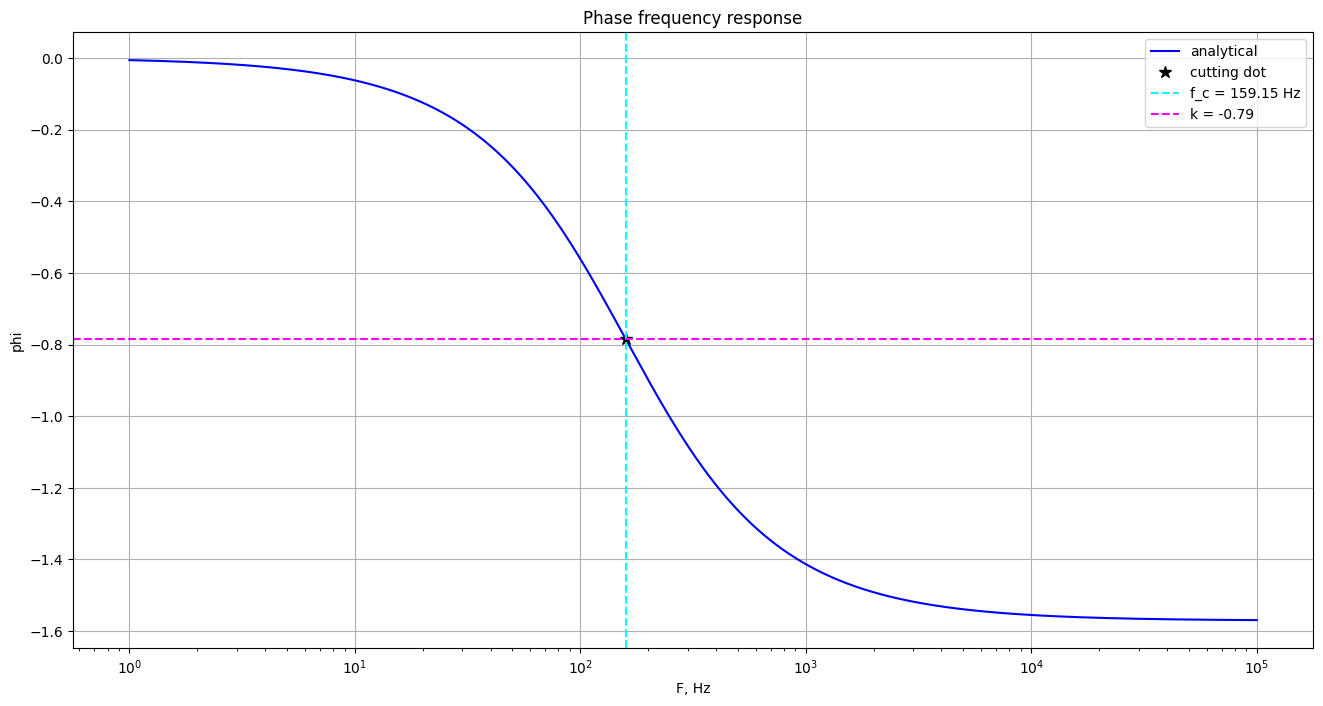
\includegraphics[width=\textwidth]{1_pfr.png}
    \caption{Фазово частотная характеристика фильтра нижних частот.}
    \label{fig:1_pfr}
\end{figure}

\subsubsection*{RC фильтр верхних частот}
\begin{figure}[H]
    \centering
    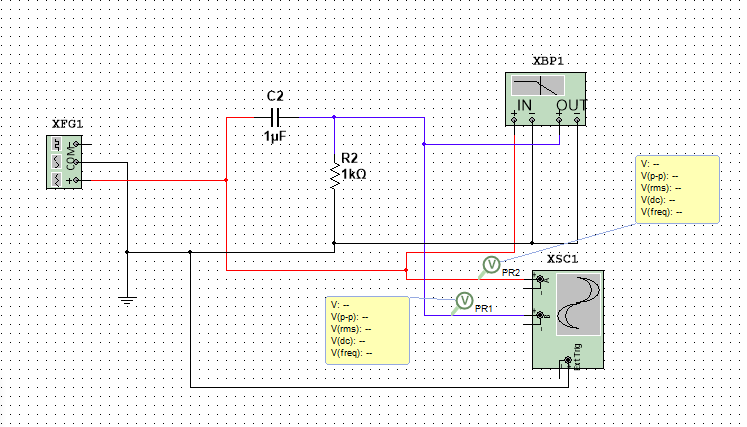
\includegraphics[width=0.5\textwidth]{2_scheme.png}
    \caption{Схема для исследования фильтра верхних частот RC.}
    \label{fig:2_scheme}
\end{figure}

На вход будем подавать синусоидальный сигнал с амплитудой $10 \ V$. \\

\begin{figure}[H]
    \centering
    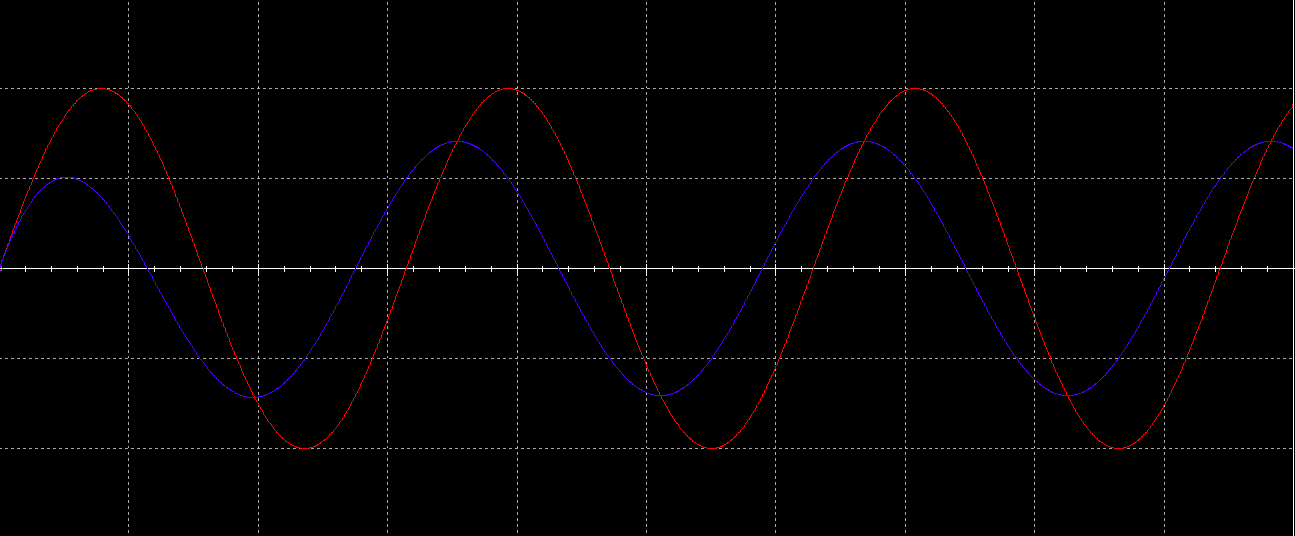
\includegraphics[width=\textwidth]{2_osc.png}
    \caption{Осциллограмма фильтра верхних частот.}
    \label{fig:2_osc}
\end{figure}

Теперь построим АЧХ и ФЧХ для данного фильтра. \\
Для этого изменяя частоту генератора синусоиды в диапазоне от $1 \ Hz$ до $100 \ kHz$ найдем 10 значений $V_{in}, \ V_{out}$ и вычислим коэффициент передачи фильтра для каждой пары и отметим данные экспериментально найденных точки на графике. \\
Также отметим частоту среза на графике и аналитически отобразим линии АЧХ и ФЧХ поверх экспериментальных точек.

\begin{figure}[H]
    \centering
    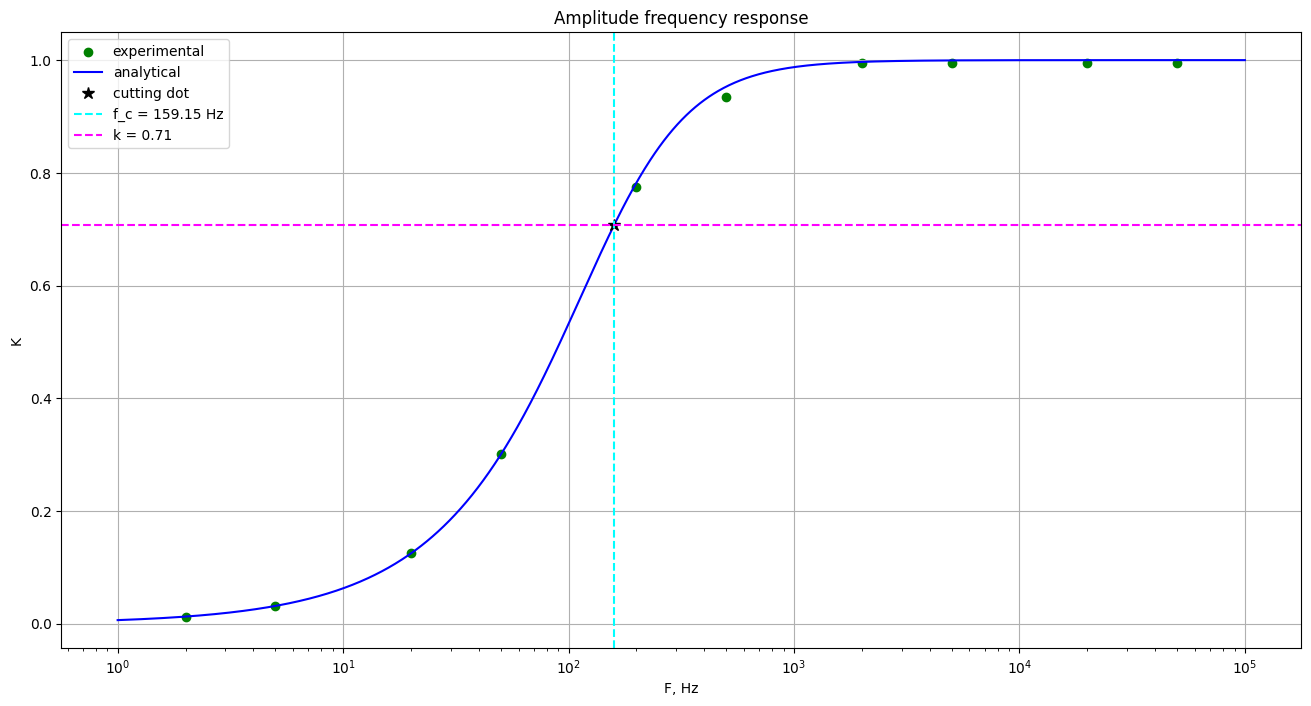
\includegraphics[width=\textwidth]{2_afr.png}
    \caption{Амплитудно частотная характеристика фильтра верхних частот.}
    \label{fig:2_afr}
\end{figure}

\begin{figure}[H]
    \centering
    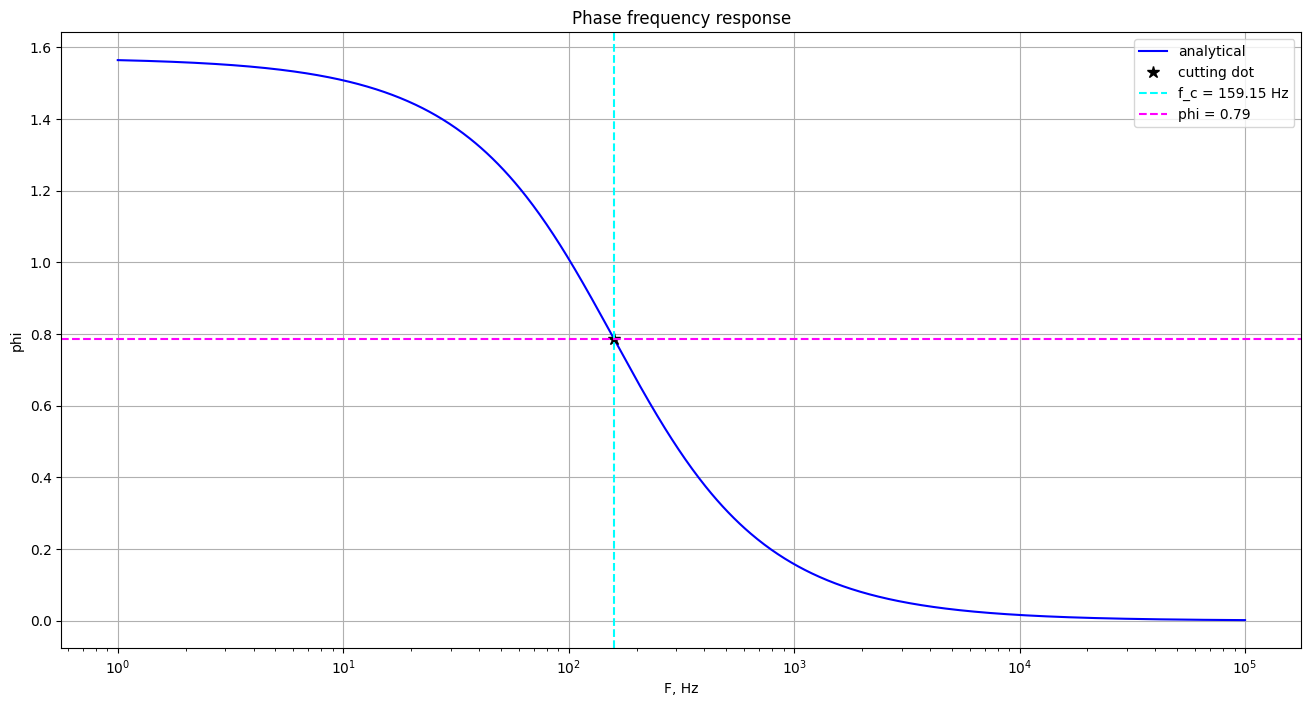
\includegraphics[width=\textwidth]{2_pfr.png}
    \caption{Фазово частотная характеристика фильтра верхних частот.}
    \label{fig:2_pfr}
\end{figure}

\subsubsection*{Полосовой (избирательный) RC фильтр}
\begin{figure}[H]
    \centering
    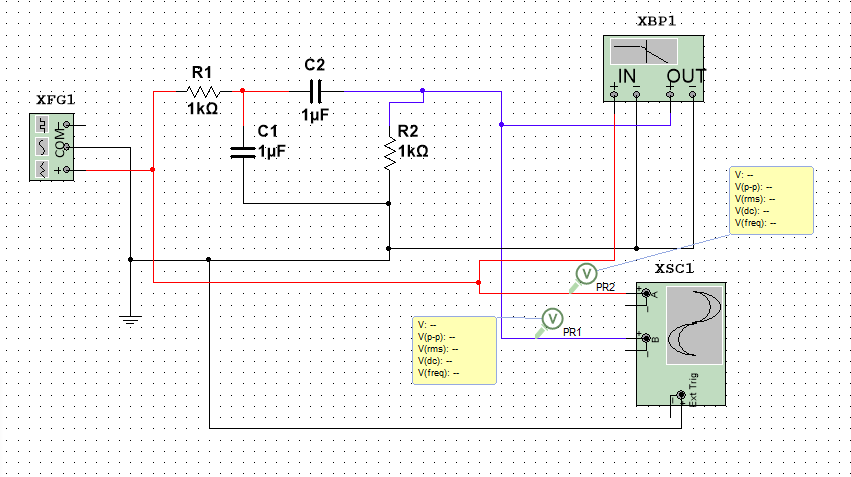
\includegraphics[width=0.5\textwidth]{3_scheme.png}
    \caption{Схема для исследования полосового (избирательного) фильтра частот RC.}
    \label{fig:3_scheme}
\end{figure}

На вход будем подавать синусоидальный сигнал с амплитудой $10 \ V$. \\

\begin{figure}[H]
    \centering
    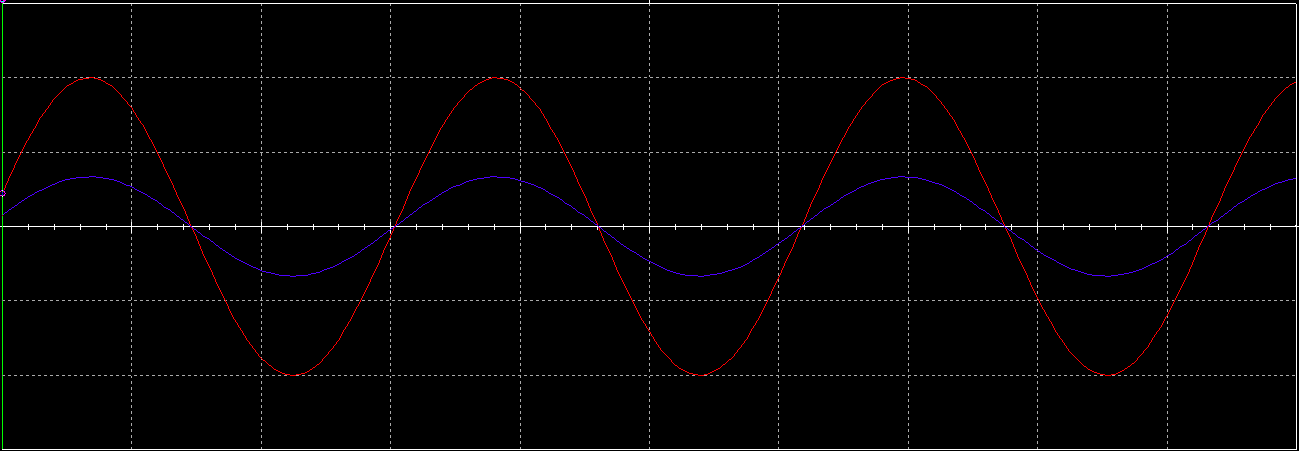
\includegraphics[width=\textwidth]{3_osc.png}
    \caption{Осциллограмма полосового (избирательного) фильтра частот RC.}
    \label{fig:3_osc}
\end{figure}

Теперь построим АЧХ и ФЧХ для данного фильтра. \\
Для этого изменяя частоту генератора синусоиды в диапазоне от $1 \ Hz$ до $100 \ kHz$ найдем 10 значений $V_{in}, \ V_{out}$ и вычислим коэффициент передачи фильтра для каждой пары и отметим данные экспериментально найденных точки на графике. \\
Также отметим частоту среза на графике и аналитически отобразим линии АЧХ и ФЧХ поверх экспериментальных точек.

\begin{figure}[H]
    \centering
    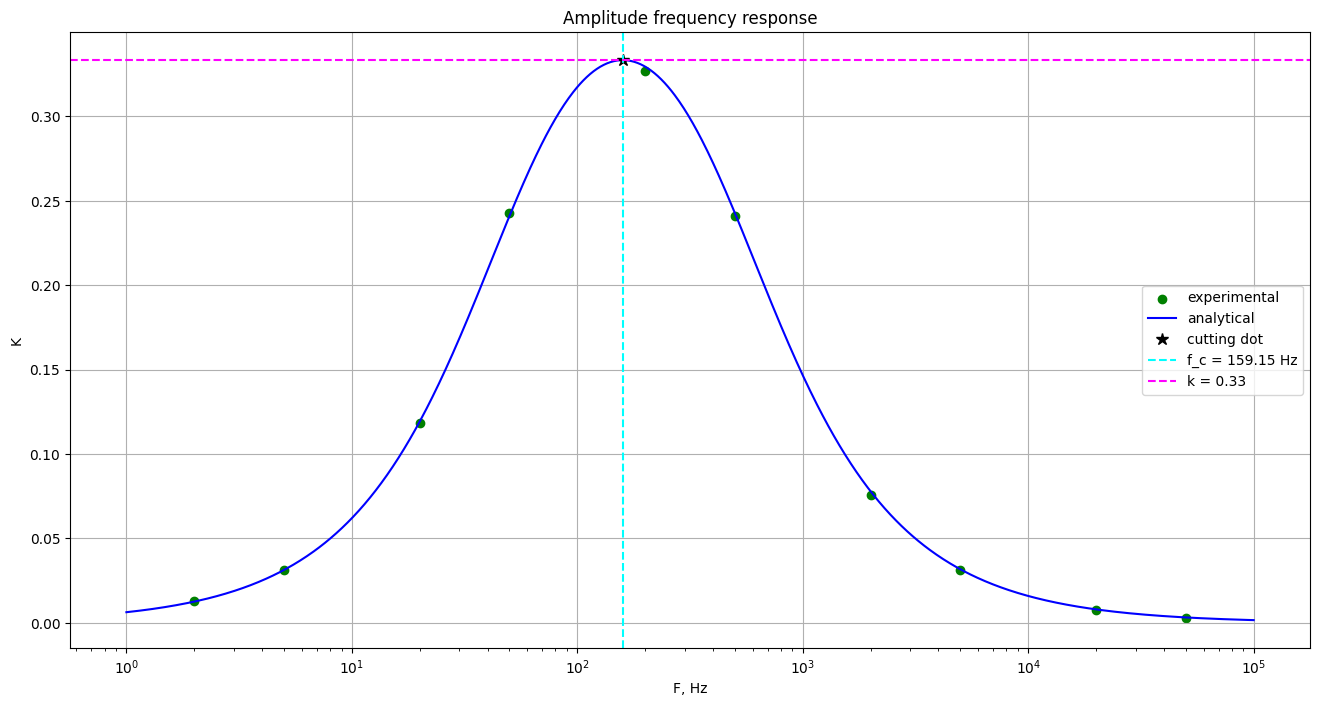
\includegraphics[width=\textwidth]{3_afr.png}
    \caption{Амплитудно частотная характеристика полосового (избирательного) фильтра частот RC.}
    \label{fig:3_afr}
\end{figure}

\begin{figure}[H]
    \centering
    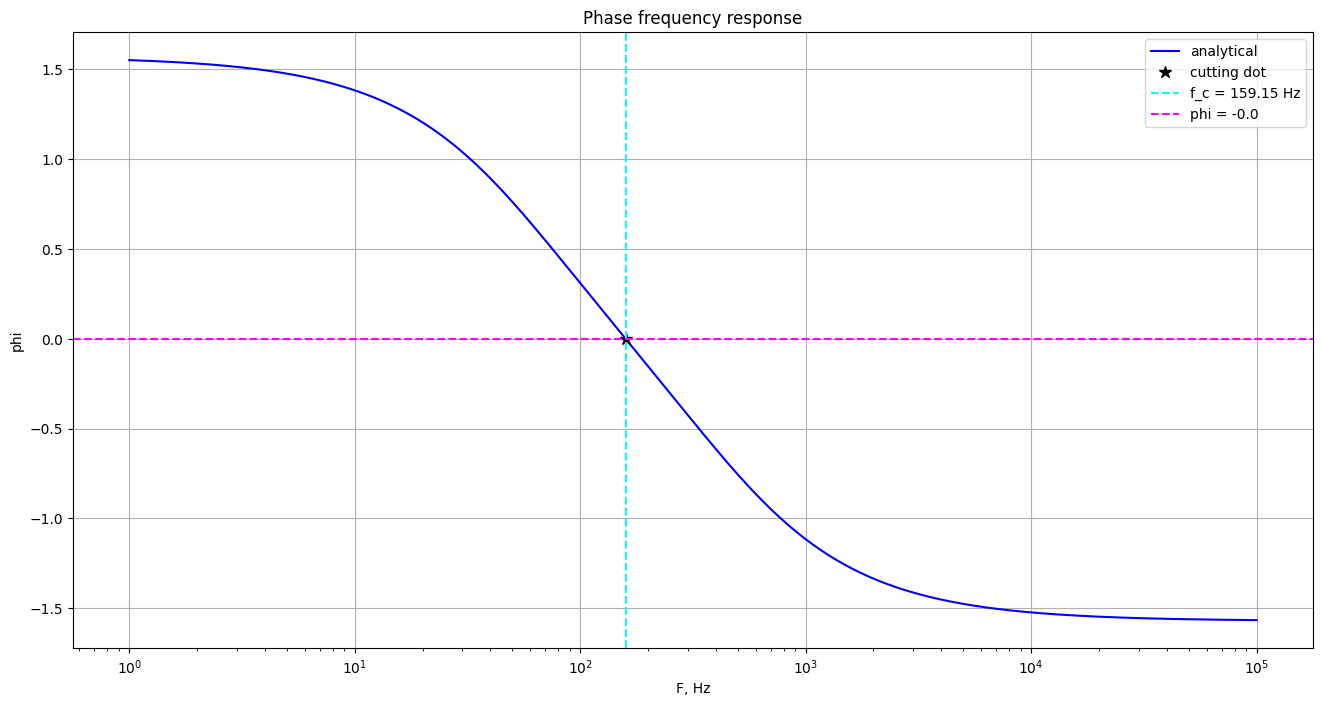
\includegraphics[width=\textwidth]{3_pfr.png}
    \caption{Фазово частотная характеристика полосового (избирательного) фильтра частот RC.}
    \label{fig:3_pfr}
\end{figure}

\subsubsection*{Полосовой (широкополосный) RC фильтр}

Рассчитаем параметры ПФ для частот среза:
\[
    f_{c_{start}} = 80 \ Hz, \ f_{c_{end}} = 15000 \ Hz \Rightarrow() \Delta = f_{c_{end}} - f_{c_{start}} = 14920 \ Hz.
\]
Вычислим центральную частоту:
\[
    f_0 = \sqrt{f_{c_{start}} \cdot f_{c_{end}}} = 1095.5 \ Hz.
\]
Определим параметры для нижней границы (фильтра верхних частот):
\[
    C_1 R_1 = \frac{1}{2 \pi f_{c_{end}}} = 0.00001 \Rightarrow C_1 = 0.01 \muF, \ R_1 = 1000 \Ohm.
\]
Определим параметры для верхней границы (фильтра нижних частот):
\[
    C_2 R_2 = \frac{1}{2 \pi f_{c_{start}}} = 0.001989 \Rightarrow C_2 = 1 \muF, \ R_2 = 1989 \Ohm.
\]

\begin{figure}[H]
    \centering
    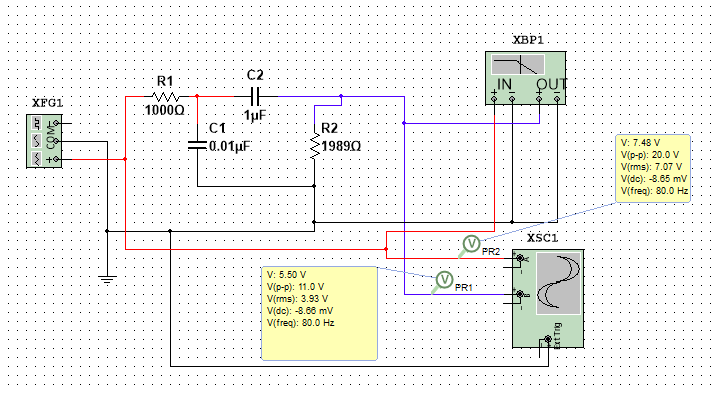
\includegraphics[width=0.5\textwidth]{4_scheme.png}
    \caption{Схема для исследования полосового (широкополосного) фильтра частот RC.}
    \label{fig:4_scheme}
\end{figure}

На вход будем подавать синусоидальный сигнал с амплитудой $10 \ V$. \\
\ \\
Приведем АЧХ (с верхними и нижними границами) построенного фильтра:
\begin{figure}[H]
    \centering
    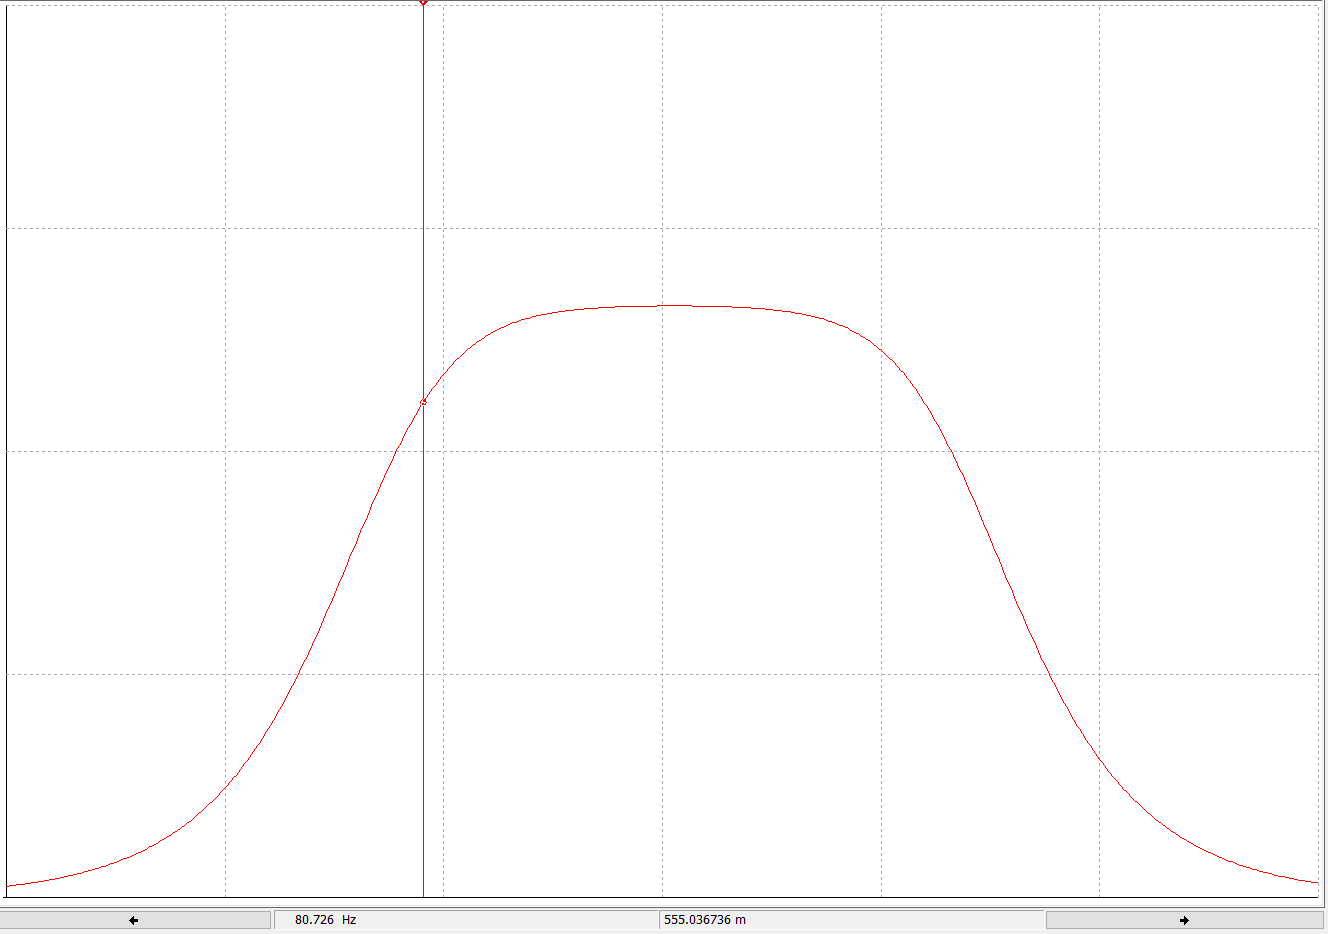
\includegraphics[width=\textwidth]{4_bode_left.png}
    \caption{Осциллограмма полосового (широкополосного) фильтра частот RC с левой границей.}
    \label{fig:4_osc_left}
\end{figure}

\begin{figure}[H]
    \centering
    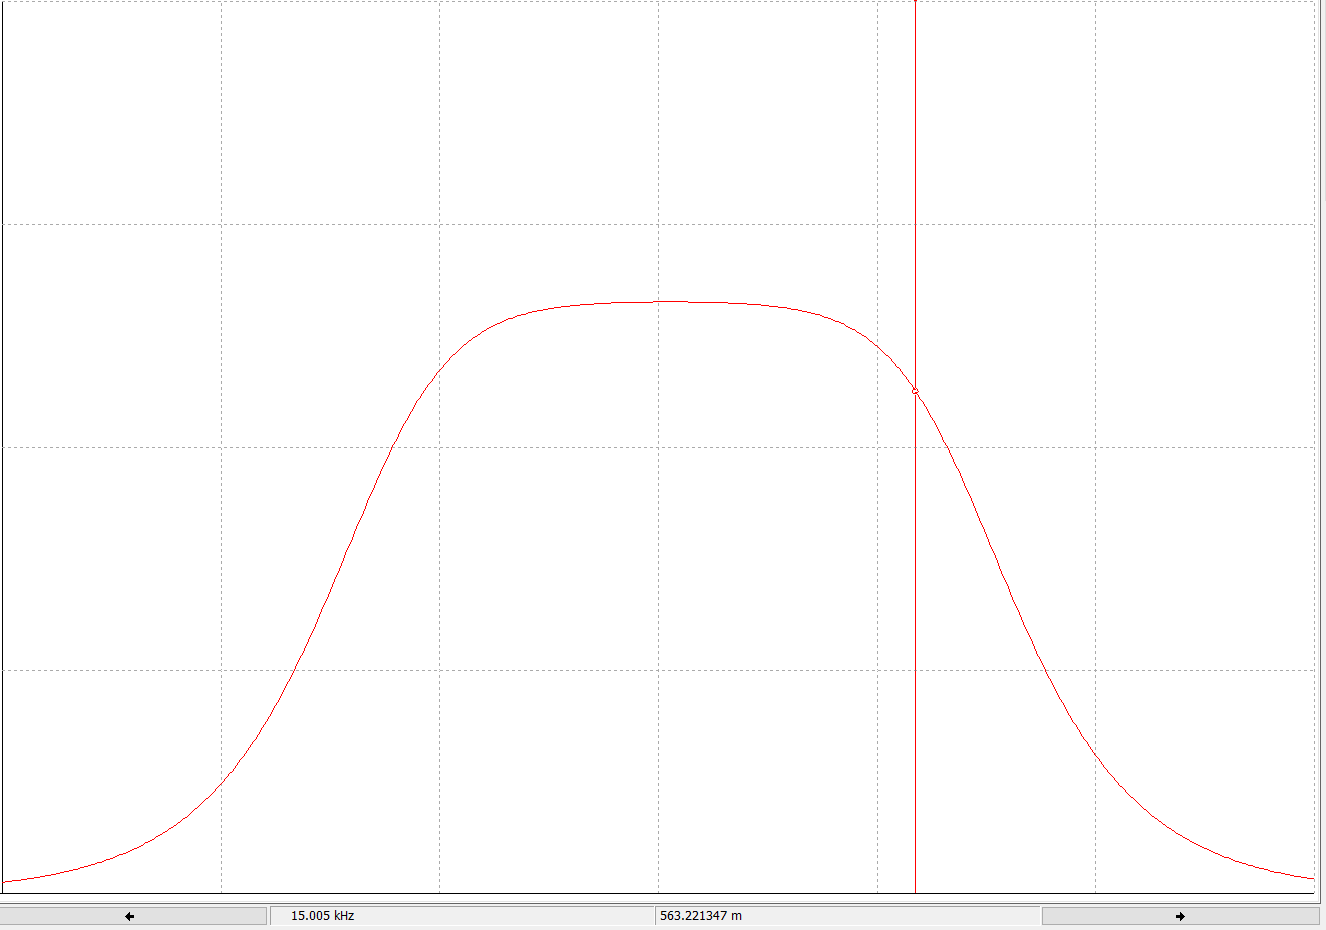
\includegraphics[width=\textwidth]{4_bode_right.png}
    \caption{Осциллограмма полосового (широкополосного) фильтра частот RC с правой границей.}
    \label{fig:4_osc_right}
\end{figure}

Как видно, расчеты сделаны верно.

\begin{figure}[H]
    \centering
    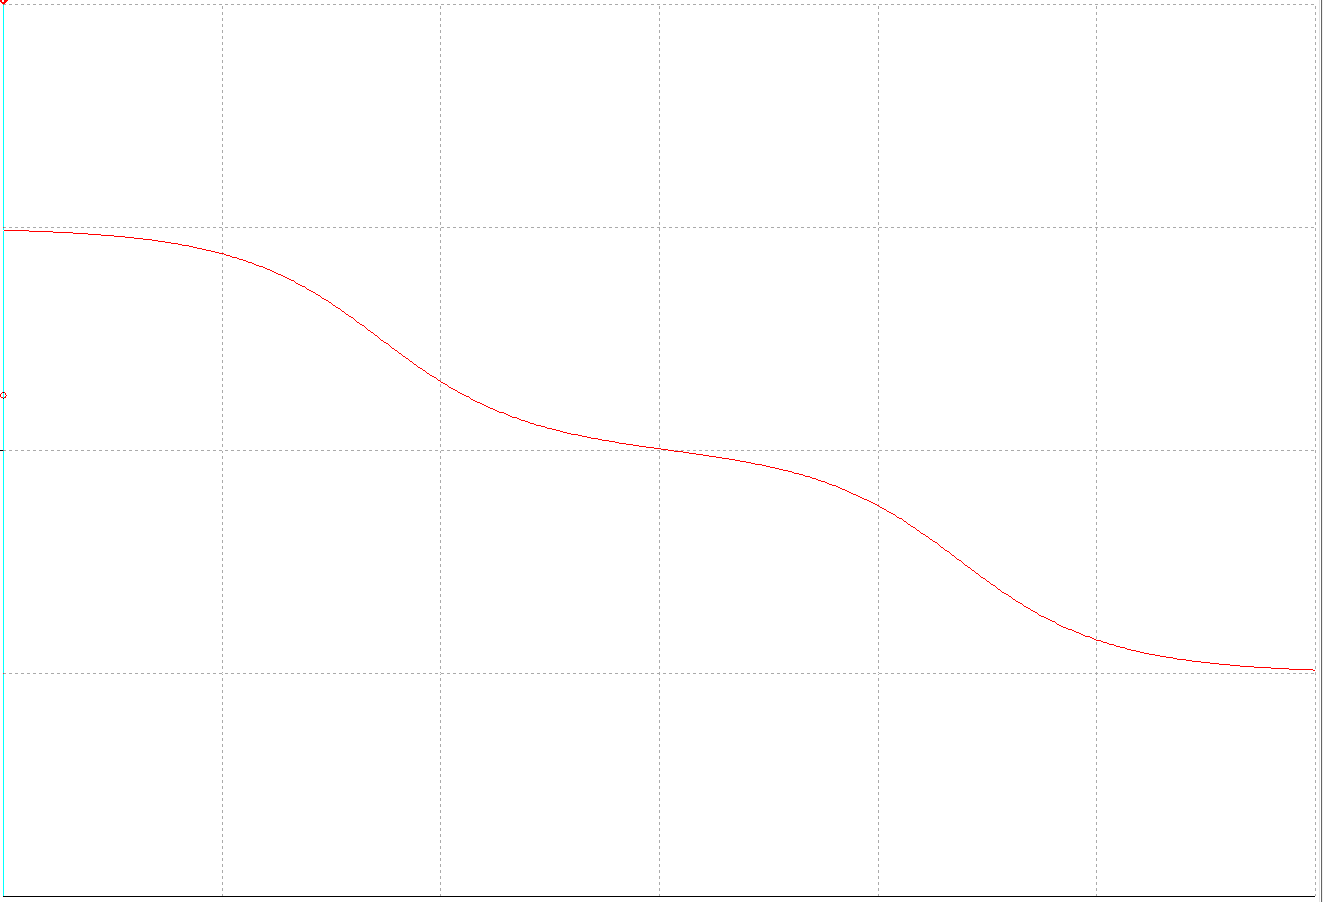
\includegraphics[width=\textwidth]{4_pfr.png}
    \caption{Фазово частотная характеристика полосового (широкополосного) фильтра частот RC.}
    \label{fig:4_pfr}
\end{figure}

\subsection*{Выводы}
В данной работе исследовались электрические фильтры. \\
Электрическим фильтром называется четырехполюсник, устанавливаемый между источником питания и нагрузкой и служащий для беспрепятственного (с малым затуханием) пропускания токов одних частот и задержки (или пропускания с большим затуханием) токов других частот.\\
Диапазон частот, пропускаемых фильтром без затухания (с малым затуханием), называется полосой пропускания или полосой прозрачности; диапазон частот, пропускаемых с большим затуханием, называется полосой затухания или полосой задерживания. Качество фильтра считается тем выше, чем ярче выражены его фильтрующие свойства, т.е. чем сильнее возрастает затухание в полосе задерживания.\\
В качестве пассивных фильтров обычно применяются четырехполюсники на основе катушек индуктивности и конденсаторов. Возможно также применение пассивных RC-фильтров, используемых при больших сопротивлениях нагрузки.\\
\ \\
В работе последовательно исследовались: фильтр нижних частот, фильтр верхних частот, полосовой (избирательный) фильтр частот, а также полосовой (широкополосный) фильтр частот. \\
Для каждого случая была сконструирована схема моделирования, найдено 10 значений входного и выходного напряжений на компоненте (при различных входных частотах). Затем были построены АЧХ и ФЧХ фильтров и найдены частоты срезов. \\

\end{document}